\section{Face representation and identification}
Approaching the face recognition challenge, we gave up manually crafted features as LBP or HOG in favour of more sophisticated ones learned by deep learning methods in a data driven way. Therefore, we employed a solution respecting the FaceNet system which, based on  deep convolutional neural network architecture, learns the mappings of faces on an 128-dimensional euclidian space where the simple L2 norm represents the similarity between faces. In order for such a system to be reliable it should prove that is, among others, pose and ilumination invariant, as well as scale, that is not prone to errors due to the quality of the image and also should be able to match faces in photos took years apart. For a lot of these challenges, the FaceNet system managed to find a way to overcome them as Schroff et all. presented in \cite{SchroffKP15}.
\begin{figure}[h]
	\begin{center}
		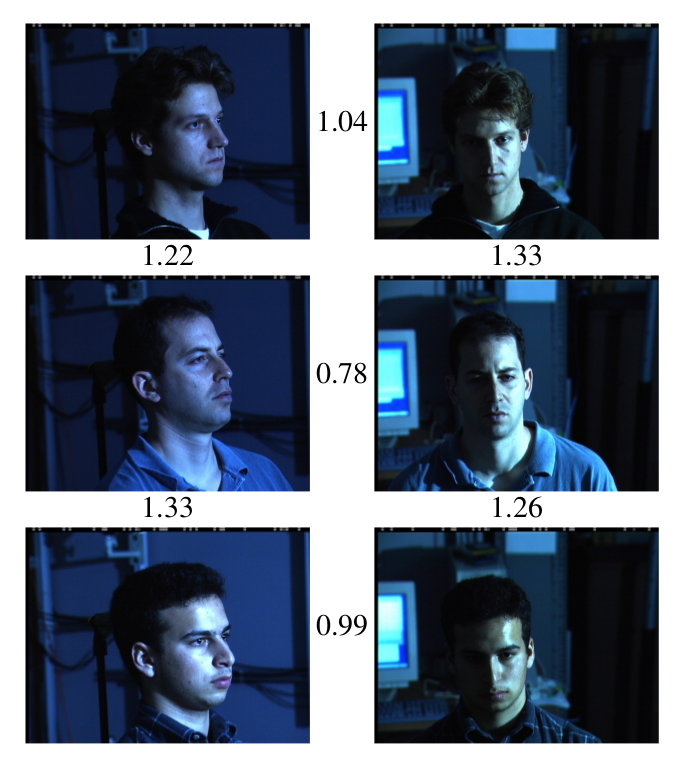
\includegraphics[width=7cm]{facenet-results}
	\end{center}
	\caption[FaceNet pose and ilumination invariance from \cite{SchroffKP15}]{Results presented in \cite{SchroffKP15} regarding the pose and ilumination invariance of the FaceNet system. As can be observed, there is a significant difference in distance between faces on the same line corresponding to the same identity and faces on different lines.}
\end{figure}
\subsection{Triplet loss}
As already stated, the FaceNet system is based on a convolutional neural network architecture. Treating the model details as a black box, the task required a form of evaluation that would reflect the desired result in the matter of face verification, recognition and clustering. As described in \cite{SchroffKP15} the target was to find an embedding $f(x)$ defined on the space of face images and into a feature space $\rm I\!R^{d}$ where the square distance between all images of the same face to be small regardless of imaging conditions and large between images of faces corresponding to different identities. Another constraint on $f(x)$ was to live on the $d$-dimensional hypersphere, meaning $||f(x)||_{2}=1$. As opposed to other losses, the triplet loss does not try to enforce the embedding on a single point but conducts the mapping of the same identity faces on a manifold while still allows a discriminative distance between faces of different identity. 

\begin{figure}[h]
	\begin{center}
		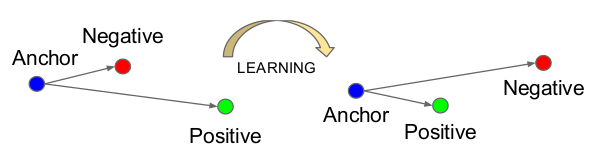
\includegraphics[width=15cm]{triplet-loss}
	\end{center}
	\caption[Triplet loss visualisation]{Visual representation of the triplet loss as presented in \cite{SchroffKP15}. It exemplifies how, through the process of learning, faces of the same identity (anchor and positive) are brought closer while faces of different identities (anchor and negative) are drifted apart }
\end{figure}

In other words, the purpose of the triplet loss is to ensure that an anchor image $x_{i}^{a}$ of a face is closer to all other images of the same face $x_{i}^{p}$ than any other image of different identity face $x_{i}^{n}$. This can be written as
\begin{align}
	||x_{i}^{a}  - x_{i}^{p} ||_{2} + \alpha < ||x_{i}^{a}  - x_{i}^{n} ||_{2}, \ \ \forall (x_{i}^{a}, x_{i}^{p}, x_{i}^{n}) \in \Psi
\end{align} where $\Psi$ is the set of all triplets from the training data, and $\alpha$ is a control parameter that imposes a minimum distance between faces of different identities. From this equation, Schroff et al. formulate in \cite{SchroffKP15} the loss that was being minimized as 
\begin{align}
L = \sum_{i}^{N} [||f(x_{i}^{a}) - f(x_{i}^{p})||_{2}^{2} - ||f(x_i^a) - f(x_i^n)||_{2}^{2} + \alpha]_{+}
\end{align}
\textbf{Here I could write more about the triplet selection}

\subsection{CNN architecture}
There were two Convolutional Network Architectures that the FaceNet experimented with: first one was based on Zeiller\&Fergus \cite{ZeilerF13} to which, based on \cite{LinCY13}, Schroff et al. added $1 \times 1 \times d$ convolutional layers between the standards convolutional layers, resulting in 22 layers deep model as can be seen in Table 2.1;
\begin{table}[h]
	\begin{center}
		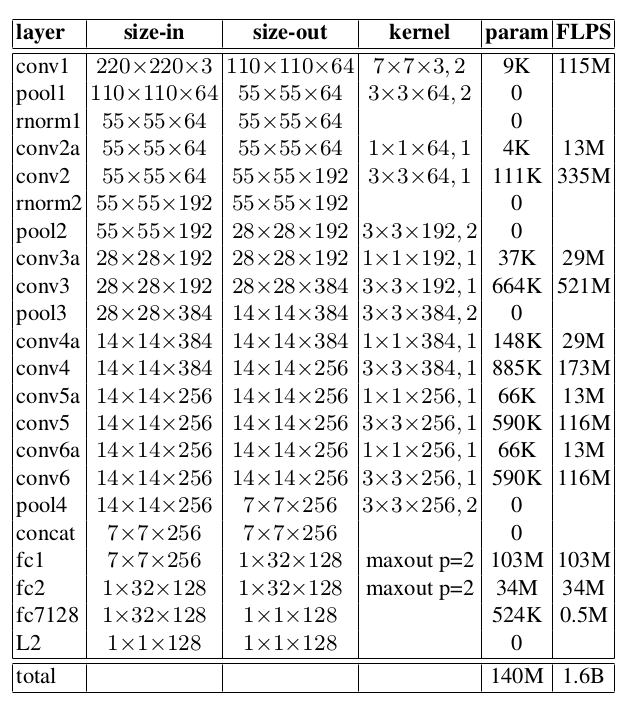
\includegraphics[width=10cm]{ZeilerFergus-architecture}
	\end{center}
	\caption[Zeiler\&Fergus architecture used in FaceNet]{Table shows the NN1 architecture from \cite{SchroffKP15} based on Zeiler\&Fergus model with $1 \times 1$ convolutions}
\end{table}
 second one was based on the GoogLeNet style Inception models \cite{DSzegedyLJSRAEVR14} which, as stated in \cite{SchroffKP15}, have $20\times$ fewer parameters and up to $5\times$fewer FLOPS. The architecture is presented in Table 2.2. In all their experiments, the CNN was trained using Stochastic Gradient Descent with standard backpropagation and AdaGrad. The training time reported in \cite{SchroffKP15} was between 1,000 to 2,000 hours on a CPU cluster and even though the decrease in loss was stated to slow down drastically after 500 hours of training, this still means that the training of such a network on a consumer used PC is infeasible. 
 \begin{table}[h]
 	\begin{center}
 		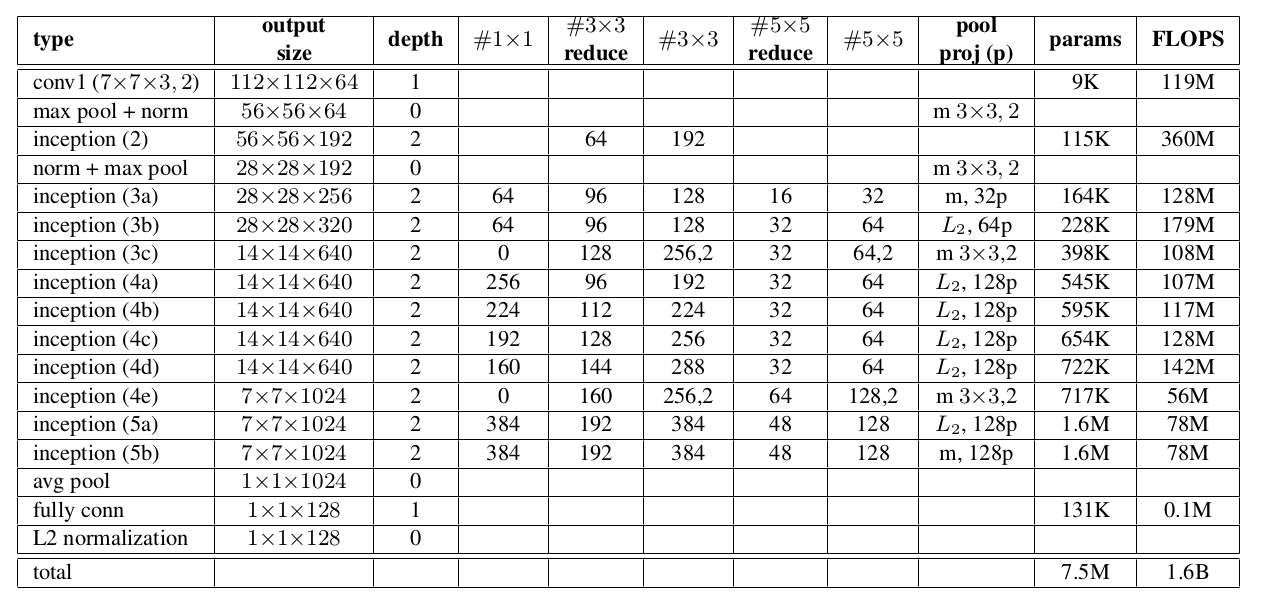
\includegraphics[width=15cm]{googlenet-architecture}
 	\end{center}
 	\caption[NN2 Inception CNN architecture]{NN2 details as presented in \cite{SchroffKP15}, the only difference to the model from \cite{DSzegedyLJSRAEVR14} is the use of $L_2$ norm instead of max pooling where specified and that the pooling is always $3\times3$}
 \end{table}
\subsection{Face identification} \label{face_recognition}

This part comes natural given the constraint that the embedding function learned by the CNN should map the face image on the surface of the 128-dimensions hypersphere of radius 1 where the Euclidean distance is a direct measure of face similarity. Therefore, having computed the feature vector of two faces, all that is left to do is to determine the Euclidean distance corresponding to those 2 points whose coordinates are represented by the elements of the feature vectors. 
The question that arises immediately is what threshold should be used when deciding if the representations correspond to the same identity? In other words, having known the identity of one face and trying to decide if the second face belongs to the same identity, what is the maximum distance between the faces representations computed by the neural network at which we can assign the identity of the first face to the second? As the embedding function, this threshold can also be learned in a data driven way like this: having a set $S$ of face images with their corresponding identities where $|S| = n$, the idea is to form pairs of faces with same and different identities and to create two histograms, one with distances between faces in pairs of the same identity and one with distances of pairs with different identities and to overlap them in order to see the point of intersection. The representation distance corresponding to this point can then be used as the threshold for determining the identity of a face.

